\chapter[Results]{Results}
\label{cp:results}

{
	\parindent0pt
	The data collected as part of the evaluation of the introduced trigger strategies is presented and discussed in this section. The hardware and software setup are given in \autoref{sec:experimental_setup}, as to allow for reproducibility of our results. Sections \ref{sec:justification_rebuild} and \ref{sec:overhead_results} discuss some implementation choices based on collected data. The main benchmark results including achieved speedups and default trigger parameters are presented in \autoref{sec:benchmarking_results}, grouped by scenario. Finally, \autoref{sec:liveinfo_benchmarks} shows statistics collected through the \texttt{LiveInfo} system, as to motivate hybrid triggers.
}


\section{Experimental Setup}
\label{sec:experimental_setup}
The measurements collected for analysis were obtained on the CoolMUC4 Linux-Cluster of the Leibniz\-/Rechenzentrum\footnote{\href{https://www.lrz.de/}{\texttt{https://www.lrz.de/}}}. The nodes in the \texttt{cm4} cluster consist of processors in the Sapphire Rapids family (Intel\textsuperscript{\textregistered} Xeon\textsuperscript{\textregistered} Platinum 8480+)  with \qty{2.1}{\gibi \byte} of memory per logical CPU and \qty{488}{\gibi \byte} per node \cite{LSC2025}. For benchmarking purposes, the AutoPas library and \texttt{md-flexible} were compiled with Spack GCC 13.2.0 and Intel MPI 2021.12.0 on commit \texttt{bc47d1ea7e8598afcf58bd35fc531439aa0c7dda}.

The scripts used to generate the Slurm jobs and configuration files can be found in the repository of this thesis\footnote{\href{https://github.com/ladnik/bachelor-thesis}{\texttt{https://github.com/ladnik/bachelor-thesis}}}.


\section{Choice of Simulation Statistics}
\label{sec:justification_rebuild}
As referred to before in \autoref{sec:avail_sim_stats}, all trigger strategies are based on the iteration runtimes excluding rebuild times. This choice can be justified by inspecting runtime data we collected: As shown  in \autoref{fig:rebuild_times}, the rebuild times change little over all iterations simulated with a particular configuration. Their inclusion therefore does not provide any new information, but rather smooths out the overall measurements and thus decreases the effectivity at which a scenario change can be detected.

Additionally, rebuild iterations only happen at \texttt{rebuildFrequency}. This can lead to stability problems in trigger strategies used with a low number of samples, as the few rebuild iterations greatly outweigh all non-rebuild iterations.

\begin{figure}[htpb]
	\centering
	\begin{subfigure}[t]{0.45\textwidth}
		\vskip0pt
		\centering
		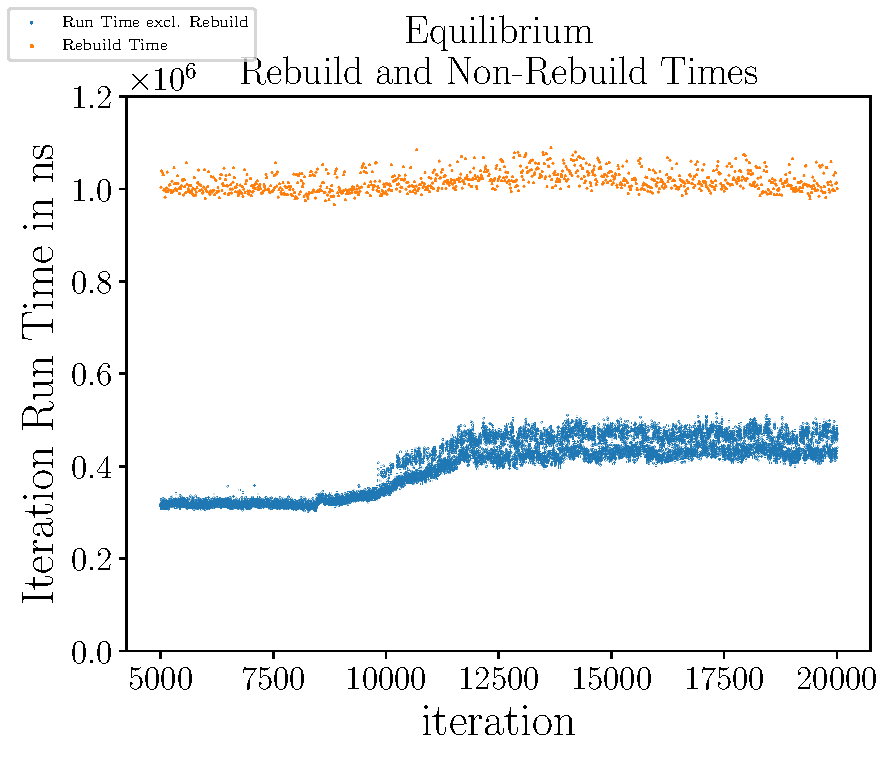
\includegraphics[width=\textwidth]{./Figures/plots/equilibrium_rebuild.pdf}
	\end{subfigure}
	\hfill
	\begin{subfigure}[t]{0.45\textwidth}
		\vskip0pt
		\centering
		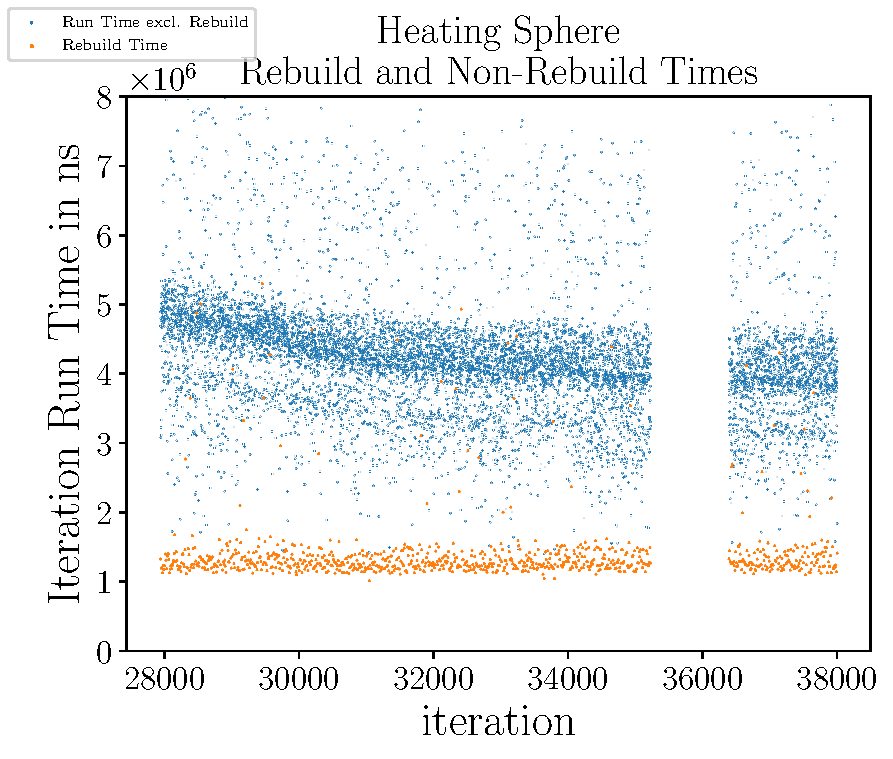
\includegraphics[width=\textwidth]{./Figures/plots/hs_rebuild.pdf}
	\end{subfigure}
	% TODO: choose different runs?
	\caption{Rebuild and non-rebuild times in the equilibrium (left) and heating-sphere (right) scenario. The configurations used were \texttt{VLC-C08-N3L-AoS-CSF1} and \texttt{LC-C04-NoN3L-AoS-CSF1} respectively. The rebuild times do not contribute any new information regarding scenario change.}
	\label{fig:rebuild_times}
\end{figure}



\section{Computational Overhead}
\label{sec:overhead_results}
The implemented tuning strategies analyze data at runtime and therefore need additional computations in each iteration. The performance impact of these should be negligible in comparison to the simulation steps, as otherwise any performance gains due to fewer tuning phases are nullified.
To quantify the overhead our strategies introduce, runs without any tuning iterations are compared, such that any changes in runtime that may occur due to different tuning phase initiation points are removed. This is achieved by using a single predefined configuration, such that no tuning takes place.

\autoref{fig:performance_comparisons} (left) shows the overhead obtained in that manner for the heating-sphere scenario using \texttt{LC-C04-N3L-AoS-CSF1} and $n=500$. To better illustrate the measurements, all values are given as relative and absolute increase in average baseline runtime per iteration.
At most, an overhead of \qty{1.9}{\percent} per iteration is seen, which can be considered insignificant. Note however, that the overhead is an absolute increase; depending on the scenario, time spent computing interactions varies, therefore the relative values change. It should also be considered, that the absolute difference between the static baseline and the dynamic runs lay in the range of \SIrange{1}{7}{\second} over the complete run. Hardware heterogeneity might make up a significant part of this difference --- which would directly influence the measured relative and absolute overhead. Nonetheless, the results may give some indication on which strategies are more compute-intensive than others. In particular, usage of the \texttt{TimeBasedSimpleTrigger} does incur nearly no runtime penalty (\qty{0.084}{\percent}), whereas the more complex trigger strategies have a correspondingly larger impact.

To exemplify the importance of optimizing the trigger routines, \autoref{fig:performance_comparisons} (right) illustrates the runtime differences between naive and optimized triggers in the equilibrium scenario. The naive version recalculates the average over all samples each iteration, whereas the optimized version uses a ring buffer and running summation to reduce computational cost.
The speedup experienced is not only due to a lowering of computational overhead, but also due to a lower number of tuning iterations. This can be explained by self influence of the triggers: Higher overhead might lead to higher fluctuation in iteration runtime which in turn leads to unstable trigger behavior, particularly in the averaging trigger. % TODO: this is not a good argument

% TODO: colors
\begin{figure}[htpb]
	\tikzset{
		barstyle1/.style={fill=tumblueaccmedium, draw=chaptertumblue},
		barstyle2/.style={pattern color=tumblueaccmedium, draw=chaptertumblue, pattern=north east lines},
	}
	\begin{subfigure}{0.45\textwidth}
		\centering
		\begin{tikzpicture}
			\def\barwidth{15pt}
			\begin{axis}[
					height=0.8\textwidth,
					width=\textwidth,
					axis y line*=left,
					xlabel={Trigger Strategy},
					ylabel={It. Overhead in \unit{\percent}},
					enlarge x limits=0.2,
					ymin=0,
					ymax=2.1,
					symbolic x coords={Simple,Avg,Split,Reg},
					xtick=data,
					bar width=\barwidth,
					legend entries={Overhead},
					legend pos=north west,
				]

				\addlegendimage{legend image code/.code={
							\draw[barstyle1, anchor=center] (0cm, -0.15cm)  rectangle (0.3cm,0.15cm);
						}}
				\addlegendentry{\scriptsize Overhead}

				% Overheads
				\addplot[ybar, barstyle1] coordinates {
						(Simple,0.084)
						(Avg,0.57)
						(Split,1.39)
						(Reg,1.9)
					};
			\end{axis}
			\begin{axis}[
					height=0.8\textwidth,
					width=\textwidth,
					axis y line*=right,
					axis x line=none,
					ymin=0, ymax=123,
					ylabel={It. Overhead in \unit{\micro\second}},
					symbolic x coords={Simple,Avg,Split,Reg},
				]
				\addplot[ybar, fill=none, draw=none] coordinates {
						(Simple,4.97)
						(Avg,33.31)
						(Split,81.64)
						(Reg,111.6)
					};
			\end{axis}
		\end{tikzpicture}
		\label{fig:overhead_comparison}
	\end{subfigure}%
	\hfill
	\begin{subfigure}{0.45\textwidth}
		\centering
		\begin{tikzpicture}
			\def\barwidth{15pt}
			\begin{axis}[
					height=0.8\textwidth,
					width=\textwidth,
					xlabel={Trigger Strategy},
					ylabel={Total Runtime in \unit{\second}},
					enlarge x limits=0.25,
					symbolic x coords={Avg,Split,Regression},
					xtick=data,
					bar width=\barwidth,
					legend entries={Unoptimized, Optimized}
				]

				\addlegendimage{legend image code/.code={
							\draw[barstyle1, anchor=center] (0cm, -0.15cm)  rectangle (0.3cm,0.15cm);
						}}
				\addlegendentry{\scriptsize Unoptimized}
				\addlegendimage{legend image code/.code={
							\draw[barstyle2, anchor=center] (0cm, -0.15cm)  rectangle (0.3cm,0.15cm);
						}}
				\addlegendentry{\scriptsize Optimized}

				% unoptimized average
				\addplot[ybar, bar shift=-0.5*\barwidth, barstyle1] coordinates {
						(Avg,1694.063817546)
						(Split,1141.728867654)
						(Regression,1112.338563086)
					};
				% optimized average
				\addplot[ybar, bar shift=0.5*\barwidth, barstyle2] coordinates {
						(Avg,962.648240758)
						(Split,999.681150940)
						(Regression,889.891999680)
					};
			\end{axis}
		\end{tikzpicture}
		\label{fig:optimization_speedup}
	\end{subfigure}
	\vspace{-4ex}
	\caption{Performance comparisons between the various trigger strategies: Relative and absolute iteration overhead in the heating-sphere scenario (left) and average runtime decrease obtained through optimizations in the equilibrium scenario (right).}
	\label{fig:performance_comparisons}
\end{figure}


\tikzset{
	linestyleA/.style={chaptertumblue, densely dotted, thick},
	linestyleB/.style={tumblueaccdark, densely dashed, thick},
	linestyleC/.style={tumblueaccmedium, solid, thick},
	linestyleD/.style={tumblueacclight, densely dashdotted, thick},
	linestyleE/.style={black, thin},
}

\pgfplotsset{
	triggerplot/.style={
			height=0.7\textwidth,
			width=\textwidth,
			xlabel={Trigger Factor $\lambda$},
			xtick={1.25, 1.5, 1.75},
			legend style={font=\small},
			legend cell align=center,
			legend columns=3,
			legend style={at={(0.5,1.03)}, anchor=south, fill=none, draw=none, align=center},
			legend image post style={xscale=0.5},
			ylabel near ticks},
	logtriggerplot/.style={
			triggerplot,
			log basis y = 10,
			log ticks with fixed point}
}




\section{Benchmarking Results}
\label{sec:benchmarking_results}
% Formula for deviation from static baseline:
% ROUND((stat_val/dyn_val - 1)*100)

The relative speedups presented in the following line charts were computed by the formula given in \eqref{eq:speedup_formula}, where $t_\text{baseline}$ represents the runtime with tuning phases at fixed intervals and $t_\text{dynamic}$ the runtime of our implementation.
\begin{equation}
	\text{S}=\frac{t_\text{baseline}}{t_\text{dynamic}}-1\label{eq:speedup_formula}
\end{equation}

For all plots showing the selected configurations for a given run, the blue scatter dots represent the runtime of that particular iteration. The colored background identifies the used configuration: same configurations map to the same color in a given plot. Gaps along the $x$-axis occur where tuning iterations have been logged --- as their runtime is not relevant for our purposes and would distort the actual runtime plot, they are not reported here. The gray dashed lines indicate the start of a new tuning phase.

%Additional plots and data can be found in the Appendix, \autoref{ap:additional_data}.
% TODO: use appendix?

\subsection{Equilibrium}
\subsubsection{Selected Runs}
\autoref{fig:equilibrium_trigger_behavior} shows two of the experimental runs in detail.
On the left hand side, a \texttt{TimeBasedAverageTrigger} with $\lambda=1.25$, $n=1000$ reliably detects scenario change. Two tuning phases are started in the initial phase, where overall iteration runtime increases. After the second tuning phase, a better configuration is found. As there is no further indication that the simulation state changes, the remaining iterations are performed using this configuration. As was explained in \autoref{subsec:scenario_equil}, it is indeed the case that no further configuration change is needed. In this run therefore, the presented trigger was beneficial.

On the right hand side, a worst-case outcome is shown. The \texttt{TimeBasedSimpleTrigger} used in that run triggered too many new tuning phases, which lead to an increase in total simulation runtime compared to the baseline run. The main reason for the overreaction lies in the implementation of the trigger: as long as the runtime of one iteration is greater than the one of its predecessor by a factor of $\lambda$ or more, a tuning phase is initiated. The few outliers in the equilibrium scenario that were averaged out in the previous example, are detrimental to this trigger strategy.


% TODO: check if plot sizes are correct in print!
\begin{figure}[htpb]
	\begin{subfigure}[t]{0.5\textwidth}
		\vskip 0pt
		\centering
		% equilibrium_dynamic_TimeBasedAverage_1.25_1000
		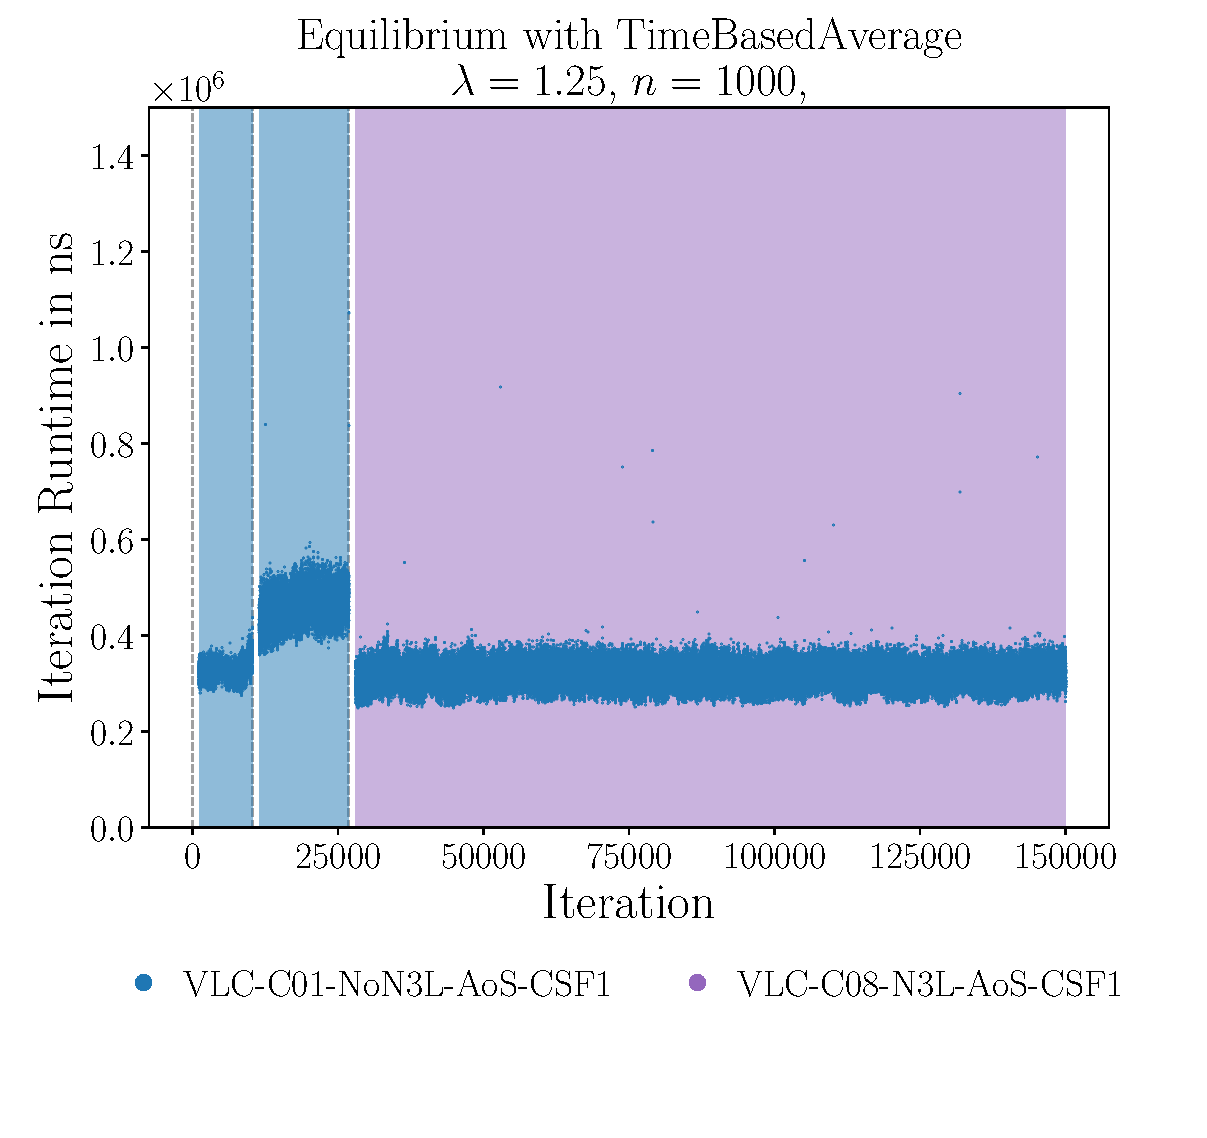
\includegraphics[width=\textwidth]{./Figures/plots/equilibrium_configs_good.pdf}
		\vspace*{-1cm}
		\subcaption{Good scenario change detection.}
	\end{subfigure}%
	\begin{subfigure}[t]{0.5\textwidth}
		\vskip 0pt
		\centering
		% equilibrium_dynamic_TimeBasedSimple_1.25_10
		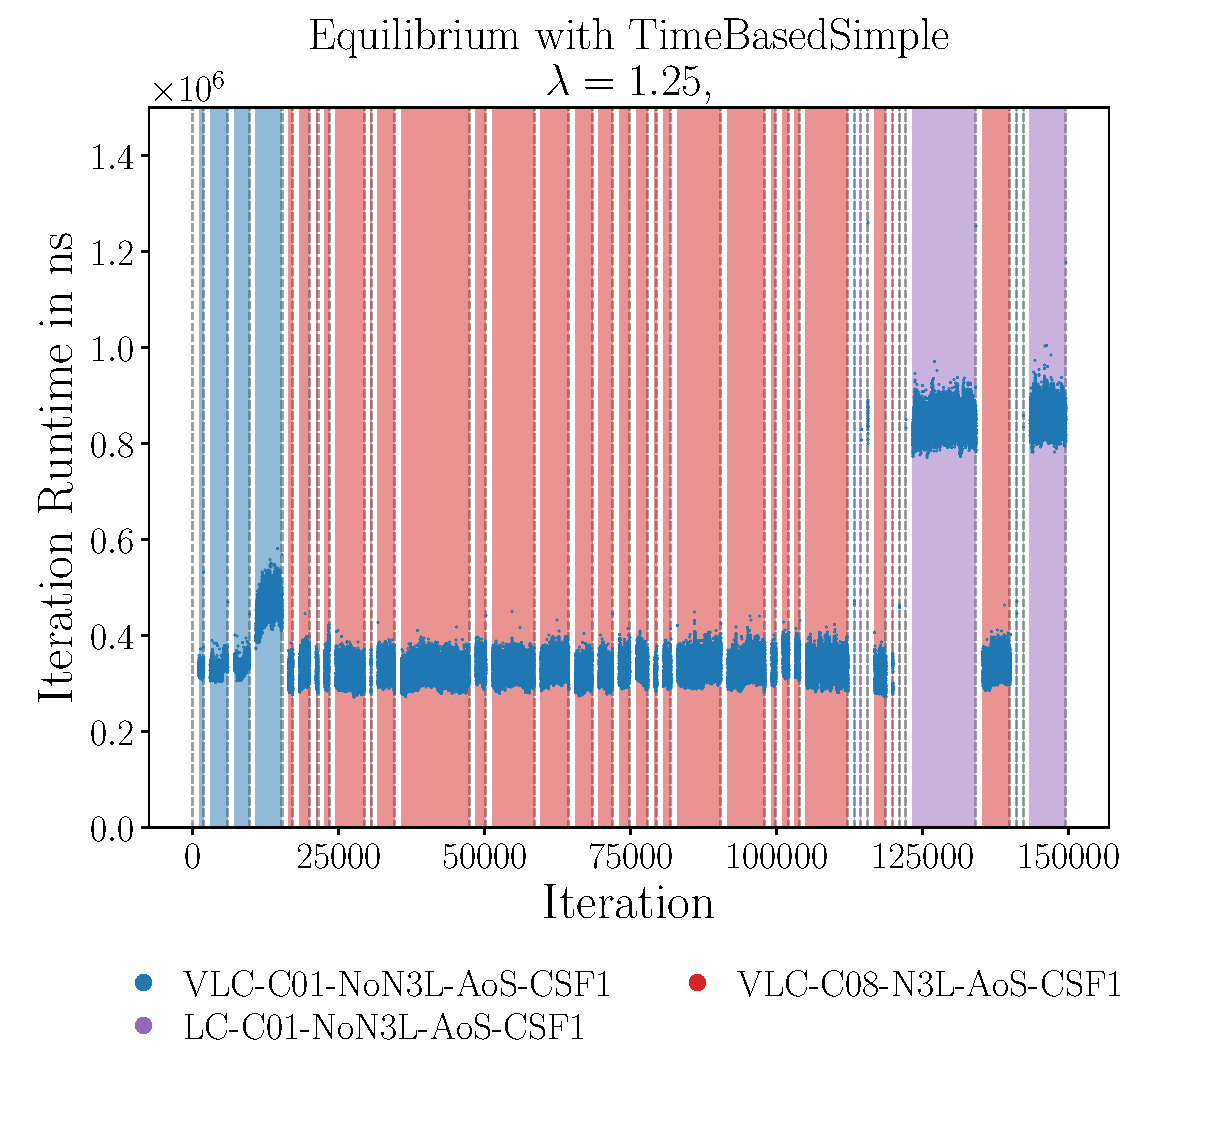
\includegraphics[width=\textwidth]{./Figures/plots/equilibrium_configs_bad.pdf}
		\vspace*{-1cm}
		\subcaption{Too many unnecessary tuning phases.}
	\end{subfigure}
	\caption{Examples of trigger behavior in the equilibrium scenario.}
	\label{fig:equilibrium_trigger_behavior}
\end{figure}



\subsubsection{Speedup and Default Parameters}

As can be seen in \autoref{fig:params_equil}, a trigger factor of $\lambda=1.5$ leads to increased speedup compared to $\lambda=1.25$ in the majority of trigger strategies. This is however mainly due to the nature of the equilibrium scenario: After the initial relaxation, the optimal configuration is not expected to change.
Therefore, not initiating any new tuning phases will lead to a decrease in total simulation runtime. That the speedup is indeed  a result of the decreased number of tuning iterations can be verified in the right-hand side plots; for the baseline run with static tuning intervals, \qty{22.6}{\percent} of iterations were spent in tuning phases.
Conversely, for strategies initiating too many new tuning intervals, i.e., with more tuning iterations than the baseline run, the simulation runtime increases.

Additionally, triggers with a larger sample size will typically trigger less frequently, as more of the variability in iteration runtime is smoothed out. For a too large number of samples such as $n>1000$, the speedup may decrease, however, as the computational overhead is directly proportional to the number of samples. This is particularly noteworthy for scenarios with fewer particles, where the computation of interactions takes less time. Therefore, the relative overhead of our strategies is larger, which would explain the lower speedup seen in the regression triggers: Compared to the \texttt{TimeBasedAverageTrigger}, at roughly the same number of tuning iterations, the speedup achieved is significantly lower.

Interestingly, the \texttt{TimeBasedSplitTrigger} with $n=250$ triggered significantly more tuning iterations for $\lambda=1.75$ than for $\lambda=1.5$.  The rather small sample size increases the sensitivity towards noise in the input data --- which is why outside influences by the underlying hardware could explain the difference between the two runs. Particularly if one considers that our equilibrium scenario consists of few particles with which interactions must be computed, resulting in low iteration runtimes.


The collected data suggests default parameters as presented in \autoref{tab:equil_defaults}.
% TODO: explain why timebasedsimple with 1.25 has fewer tuning phases

\begin{figure}[htpb]
	\centering
	\begin{subfigure}{0.45\textwidth}
		\begin{tikzpicture}
			\begin{axis}[
					triggerplot,
					legend columns=2,
					ylabel={Speedup \%},
				]
				% Baseline
				\draw[linestyleE] (axis cs:0,0) -- (axis cs: 2,0);

				% TimeBasedSimple
				\addplot[linestyleD] coordinates{
						(1.25,-5)
						(1.5,-33)
						(1.75,-32)};
				% TimeBasedAverage 1000
				\addplot[linestyleA] coordinates{
						(1.25,21)
						(1.5,44)
						(1.75,47)};
				% TimeBasedAverage 500
				\addplot[linestyleB] coordinates{
						(1.25,10)
						(1.5,34)
						(1.75,47)};
				% TimeBasedAverage 250
				\addplot[linestyleC] coordinates{
						(1.25,17)
						(1.5,26)
						(1.75,34)};
				\legend{Simple,Avg-1000,Avg-500,Avg-250}
			\end{axis}
		\end{tikzpicture}
		%		\subcaption{Simple and Average Triggers}
	\end{subfigure}
	\hspace{0.05\textwidth}
	\begin{subfigure}{0.45\textwidth}
		\begin{tikzpicture}
			\begin{axis}[
					logtriggerplot,
					legend columns=2,
					ylabel={Tuning Iterations \%},
					ymode=log,
					ymin=1,
					ymax=100,
				]
				% Baseline
				\draw[linestyleE] (axis cs:0,22.6) -- (axis cs: 2,22.6);

				% TimeBasedSimple
				\addplot[linestyleD] coordinates{
						(1.25,29.37)
						(1.5,84.88)
						(1.75,83.86)};
				% TimeBasedAverage 500
				\addplot[linestyleB] coordinates{
						(1.25,2.26)
						(1.5,2.26)
						(1.75,1.51)};
				% TimeBasedAverage 250
				\addplot[linestyleC] coordinates{
						(1.25,2.26)
						(1.5,1.51)
						(1.75,1.51)};
				% TimeBasedAverage 1000 (drawn over Avg-250)
				\addplot[linestyleA] coordinates{
						(1.25,2.26)
						(1.5,1.51)
						(1.75,1.51)};
				\legend{Simple,Avg-500,Avg-250,Avg-1000}
			\end{axis}
		\end{tikzpicture}
		%		\subcaption{Simple and Average Triggers}
	\end{subfigure}
	\begin{subfigure}{0.45\textwidth}
		\begin{tikzpicture}
			\begin{axis}[
					triggerplot,
					ylabel={Speedup \%},
				]
				% Baseline
				\draw[linestyleE] (axis cs:0,0) -- (axis cs: 2,0);

				% TimeBasedSplit 1000
				\addplot[linestyleA] coordinates{
						(1.25,42)
						(1.5,46)
						(1.75,35)};
				% TimeBasedSplit 500
				\addplot[linestyleB] coordinates{
						(1.25,43)
						(1.5,38)
						(1.75,40)};
				% TimeBasedSplit 250
				\addplot[linestyleC] coordinates{
						(1.25,-6)
						(1.5,28)
						(1.75,-7)};
				\legend{Split-1000,Split-500,Split-250}
			\end{axis}
		\end{tikzpicture}
		%		\subcaption{Split Trigger}
	\end{subfigure}
	\hspace{0.05\textwidth}
	\begin{subfigure}{0.45\textwidth}
		\begin{tikzpicture}
			\begin{axis}[
					logtriggerplot,
					ylabel={Tuning Iterations \%},
					ymode=log,
					ymin=1,
					ymax=100,
				]
				% Baseline
				\draw[linestyleE] (axis cs:0,22.6) -- (axis cs: 2,22.6);

				% TimeBasedSplit 1000
				\addplot[linestyleA] coordinates{
						(1.25,3.77)
						(1.5,3.01)
						(1.75,3.77)};
				% TimeBasedSplit 500
				\addplot[linestyleB] coordinates{
						(1.25,4.52)
						(1.5,4.52)
						(1.75,3.77)};
				% TimeBasedSplit 250
				\addplot[linestyleC] coordinates{
						(1.25,81.7)
						(1.5,6.03)
						(1.75,81.9)};
				\legend{Split-1000,Split-500,Split-250}
			\end{axis}
		\end{tikzpicture}
		%		\subcaption{Split Trigger}
	\end{subfigure}
	\begin{subfigure}{0.45\textwidth}
		\begin{tikzpicture}
			\begin{axis}[
					triggerplot,
					legend columns=2,
					ylabel={Speedup \%},
				]
				% Baseline
				\draw[linestyleE] (axis cs:0,0) -- (axis cs: 2,0);

				% TimeBasedRegression 2000
				\addplot[linestyleA] coordinates{
						(1.25,-3)
						(1.5,13)
						(1.75,14)};

				% TimeBasedRegression 1500
				\addplot[linestyleB] coordinates{
						(1.25,-4)
						(1.5,14)
						(1.75,15)};

				% TimeBasedRegression 1000
				\addplot[linestyleC] coordinates{
						(1.25,7)
						(1.5,15)
						(1.75,14)};

				% TimeBasedRegression 500		
				\addplot[linestyleD] coordinates{
						(1.25,5)
						(1.5,16)
						(1.75,15)};

				\legend{Reg-2000,Reg-1500,Reg-1000,Reg-500}
			\end{axis}
		\end{tikzpicture}
		%		\subcaption{Regression Trigger}
	\end{subfigure}%
	\hspace{0.05\textwidth}
	\begin{subfigure}{0.45\textwidth}
		\begin{tikzpicture}
			\begin{axis}[
					logtriggerplot,
					legend columns=2,
					ylabel={Tuning Iterations \%},
					ymode=log,
					ymin=1,
					ymax=100,
				]
				% Baseline
				\draw[linestyleE] (axis cs:0,22.6) -- (axis cs: 2,22.6);

				% TimeBasedRegression 2000
				\addplot[linestyleA] coordinates{
						(1.25,18.72)
						(1.5,4.32)
						(1.75,1.44)};

				% TimeBasedRegression 1500
				\addplot[linestyleB] coordinates{
						(1.25,19.37)
						(1.5,1.44)
						(1.75,1.44)};

				% TimeBasedRegression 1000
				\addplot[linestyleC] coordinates{
						(1.25,7.88)
						(1.5,1.44)
						(1.75,1.44)};

				% TimeBasedRegression 500		
				\addplot[linestyleD] coordinates{
						(1.25,10.08)
						(1.5,1.44)
						(1.75,1.44)};

				\legend{Reg-2000,Reg-1500,Reg-1000,Reg-500}
			\end{axis}
		\end{tikzpicture}
		%		\subcaption{Regression Trigger}
	\end{subfigure}%
	\caption{Trigger behavior in the equilibrium scenario, the numbers in the legends refer to the number of samples $n$ considered. The line in the background represents the baseline run. Note the logarithmic scale in the plots on the right hand side.}
	\label{fig:params_equil}
\end{figure}
\begin{table}[htpb]
	\centering
	\begin{tabular}{lcc}
		\toprule
		\textbf{Trigger}             & \textbf{Trigger factor $\lambda$} & \textbf{Number of samples $n$} \\ [0em]
		\midrule
		\texttt{TimeBasedSimple}     & not recommended                            & --                             \\
		\texttt{TimeBasedAverage}    & $1.75$                            & 500                            \\
		\texttt{TimeBasedSplit}      & $1.5$                             & 1000                           \\
		\texttt{TimeBasedRegression} & $1.5$                             & 500                            \\
		\bottomrule
	\end{tabular}
	\caption{Suggested default parameters for the equilibrium scenario.}
	\label{tab:equil_defaults}
\end{table}





\subsubsection{Optimality}
Our second evaluation metric, as stated in \autoref{sec:metrics}, concerns the quality of the chosen configurations. For efficient computation, we expect the configuration at any non-tuning iteration to be one of the best choices. As can be seen in \autoref{fig:equilibrium_optimality}, this is achieved across all strategies except the simple trigger, with all configurations being one of the top three choices for that specific iteration. It should be noted, that the ranking of optimal configurations is only an approximation, as it is based on the baseline run and therefore restricted to the resolution of that run's \texttt{tuning-interval}. The best performing strategy regarding optimality seems to be  the  \texttt{TimeBasedAverageTrigger}.

\begin{figure}[htpb]
	\begin{subfigure}{0.5\textwidth}
		\centering
		\begin{tikzpicture}
			\tikzset{
				barstyle1/.style={pattern color=tumblueaccmedium, draw=chaptertumblue,  pattern=crosshatch dots},
				barstyle2/.style={pattern color=tumblueaccmedium, draw=chaptertumblue, pattern=north east lines},
				barstyle3/.style={fill=tumblueaccmedium, draw=chaptertumblue},
				barstyle4/.style={pattern color=tumblueaccmedium, draw=chaptertumblue, pattern=vertical lines},
			}
			\def\barwidth{15pt}
			\begin{axis}[
					ybar stacked,
					height=0.8\textwidth,
					enlargelimits=0.15,
					ylabel={Selected Configuration in \unit{\percent}},
					xlabel={Trigger Strategy},
					symbolic x coords={Simple,Avg,Split,Reg},
					xtick=data,
					bar width=\barwidth,
					%				legend cell align=left,
					%				legend columns=1,
					%				legend style={at={(1.03,0.5)}, anchor=west, fill=none, draw=none, align=left},
					legend style={font=\small},
					legend cell align=center,
					legend columns=2,
					legend style={at={(0.5,1.03)}, anchor=south, fill=none, draw=none, align=center},
				]
				% TODO: align legend labels

				% Top 1
				\addplot+[ybar, barstyle3] plot coordinates {(Simple,81) (Avg,92)
						(Split,10) (Reg,10)};

				% Top 2
				\addplot+[ybar, barstyle2] plot coordinates {(Simple,2) (Avg,7)
						(Split,63) (Reg,63)};

				% Top 3
				\addplot+[ybar, barstyle4] plot coordinates {(Simple,0) (Avg,1)
						(Split,27) (Reg,27)};

				% Other
				\addplot+[ybar, barstyle1] plot coordinates {(Simple,17) (Avg,0)
						(Split,0) (Reg,0)};

				\legend{Best,Second-Best,Third-Best,Other}
			\end{axis}
		\end{tikzpicture}
	\end{subfigure}%
	\begin{subfigure}{0.5\textwidth}
		\centering
		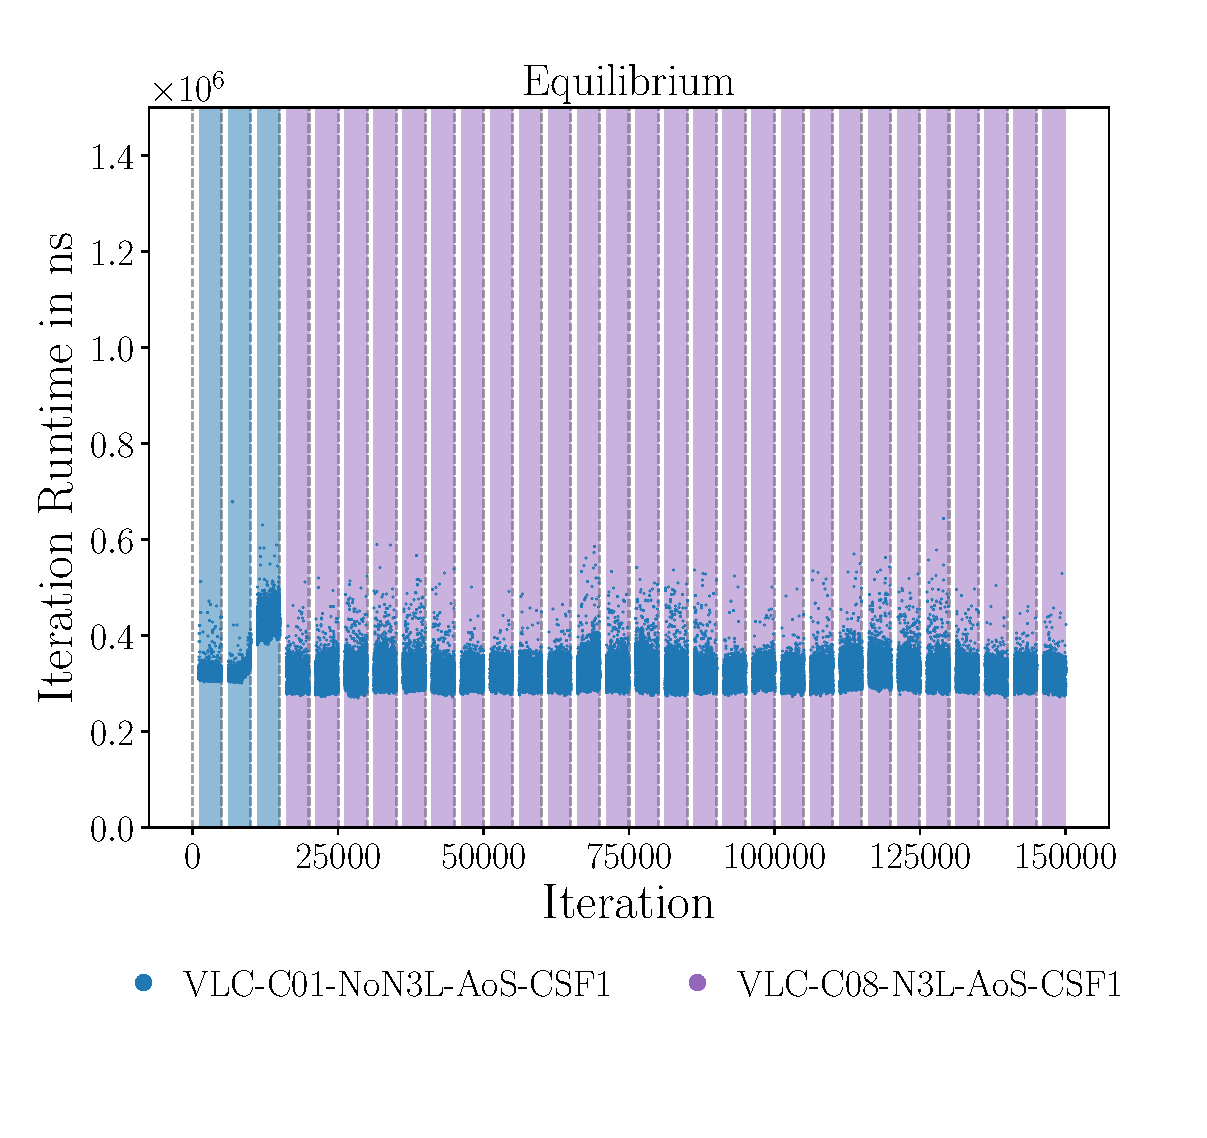
\includegraphics[width=\textwidth]{./Figures/plots/equilibrium_configs_static.pdf}
		\vspace*{-1.1cm}
	\end{subfigure}
	\caption{Ranking of configurations selected by the best run in the equilibrium scenario for each trigger strategy (left) and selected configurations in the baseline run (right).}
	\label{fig:equilibrium_optimality}
\end{figure}


\subsection{Exploding Liquid}
\subsubsection{Selected Runs}
The exploding-liquid scenario was executed using 6 MPI processees, with the simulation domain split up along the $y$-axis. This has the effect, that different ranks encounter the particle \enquote{wave} at different points in time, as it spreads from the center outwards (cf. \autoref{subsec:scenario_expl}). This can be seen in \autoref{fig:expl_trigger_behavior}, where the plot showing rank 2 (in the center of the domain, plot on right hand side) experiences high iteration runtimes at the beginning of the simulation. Rank 0 (plot on the left hand side), however, shows this influx of particles beginning not until iteration \num{50000}.
% good: exploding-liquid_dynamic_TimeBasedSplit_1.5_1000 (Rank 0)
% bad (shows magnitude should be considered): exploding-liquid_dynamic_TimeBasedSplit_1.5_1000 (Rank 2)

% alternatives:
% good: exploding-liquid_dynamic_TimeBasedSplit_1.25_1000 (Rank 0)
% good: exploding-liquid_dynamic_TimeBasedSplit_1.25_250 (Rank 0)

\begin{figure}[htpb]
	\begin{subfigure}[t]{0.5\textwidth}
		\vskip 0pt
		\centering
		% equilibrium_dynamic_TimeBasedAverage_1.25_1000
		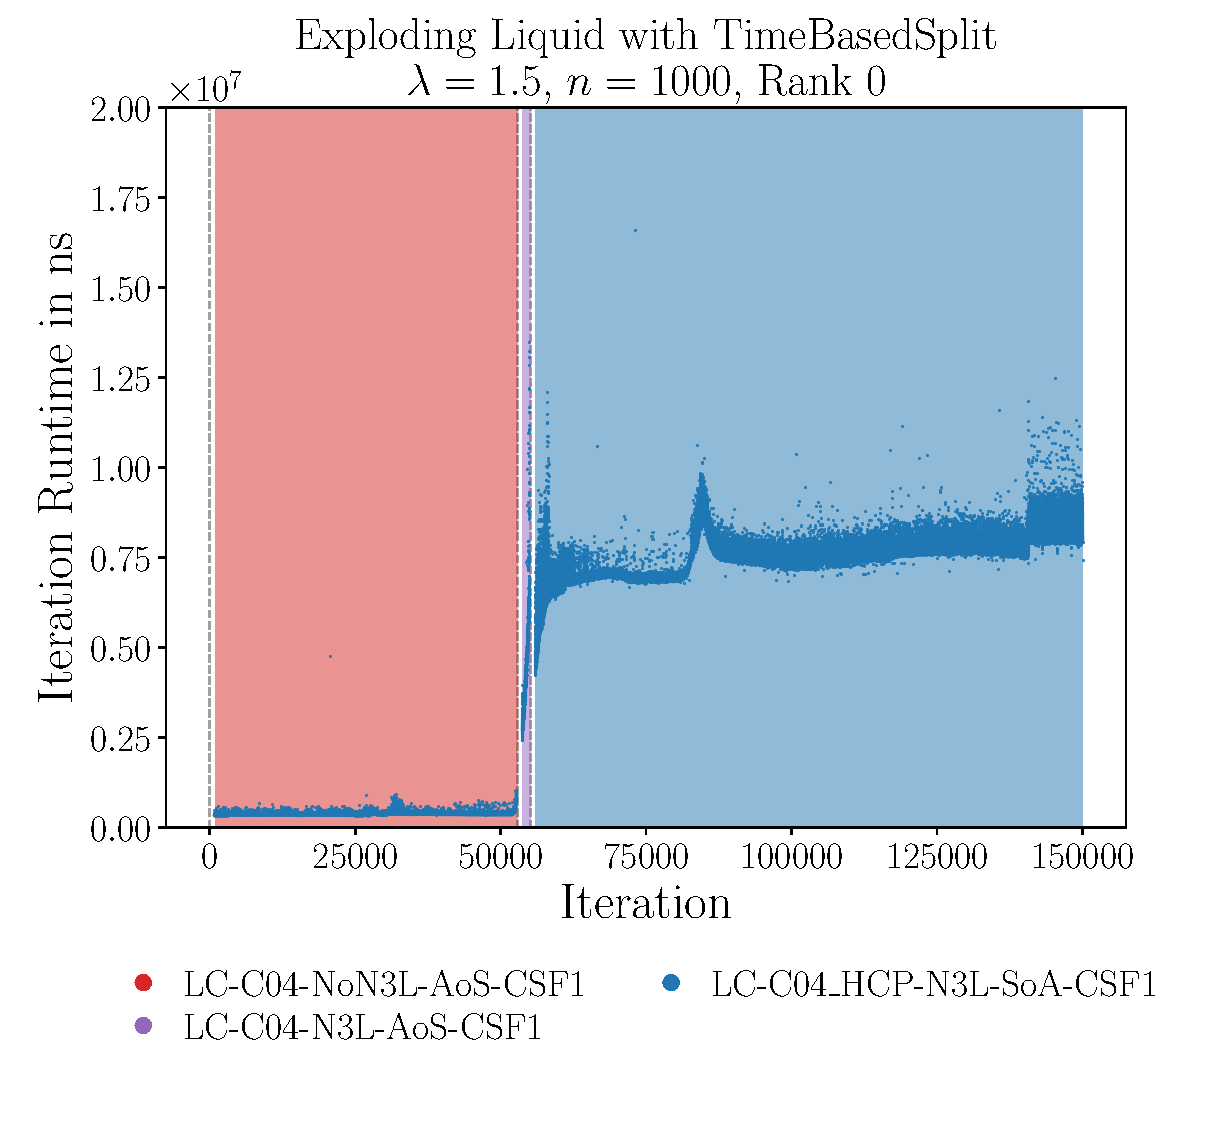
\includegraphics[width=\textwidth]{./Figures/plots/exploding-liquid_configs_good.pdf}
		\vspace*{-1cm}
		\subcaption{Good scenario change detection.}
	\end{subfigure}%
	\begin{subfigure}[t]{0.5\textwidth}
		\vskip 0pt
		\centering
		% equilibrium_dynamic_TimeBasedSimple_1.25_10
		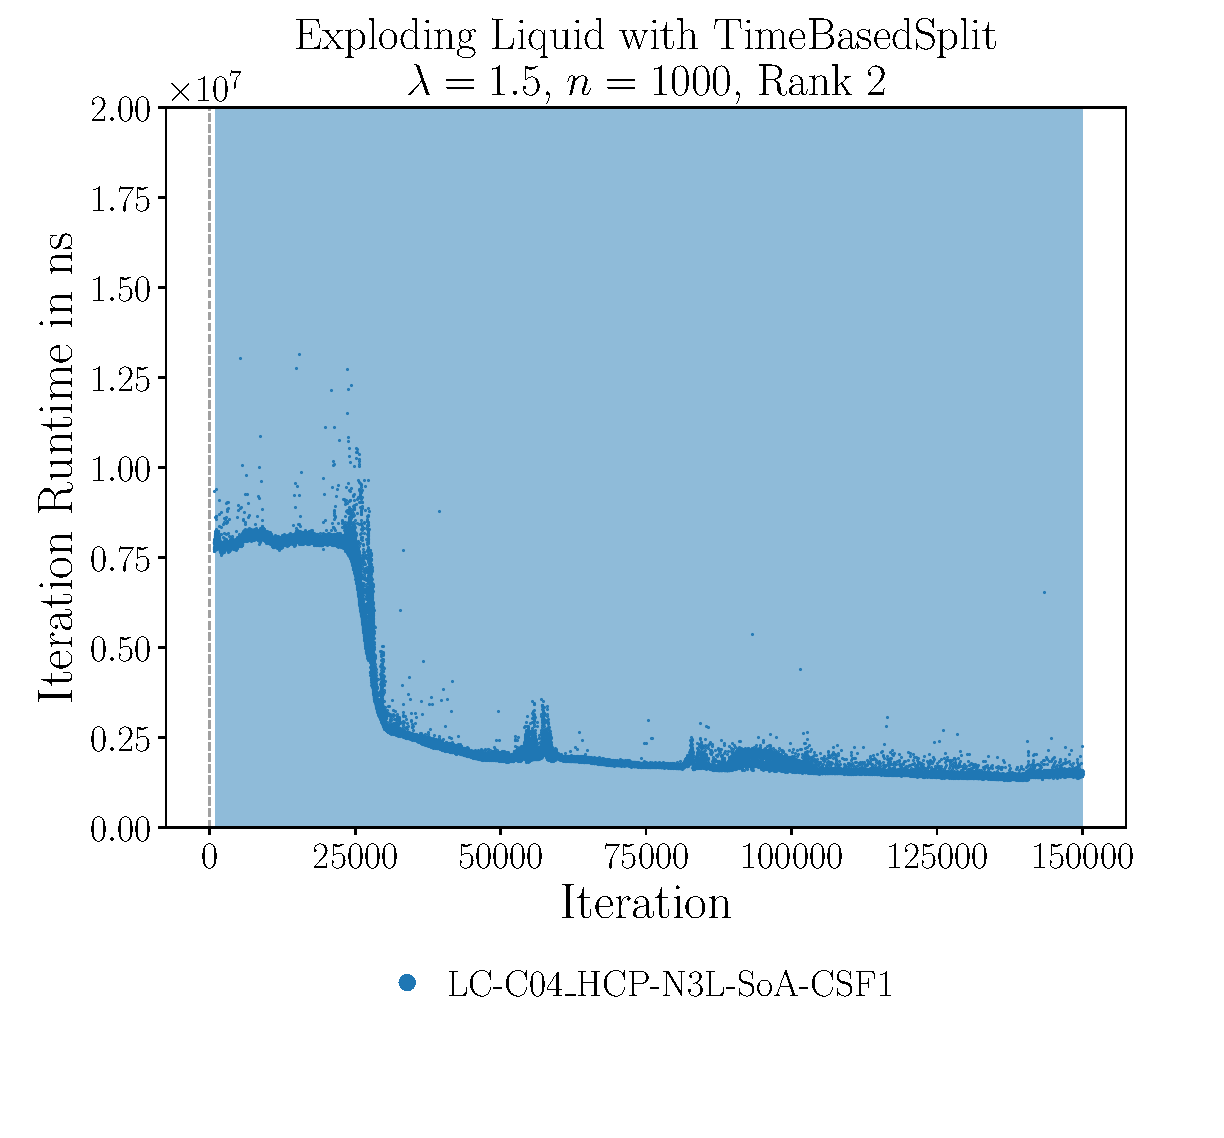
\includegraphics[width=\textwidth]{./Figures/plots/exploding-liquid_configs_bad.pdf}
		\vspace*{-1cm}
		\subcaption{No reconfiguration after peak.}
	\end{subfigure}
	\caption{Examples of trigger behavior in the exploding-liquid scenario.}
	\label{fig:expl_trigger_behavior}
\end{figure}

\subsubsection{Speedup and Default Parameters}
\subsubsection{Optimality}


\subsection{Heating Sphere}
\subsubsection{Selected Runs}
%TODO: fix axes size
\autoref{fig:hs_trigger_behavior} again presents two sample runs to illustrate optimal and unsatisfactory results. The left figure shows a reduction in the number of tuning phases initiated by the \texttt{TimeBasedAverageTrigger}. After the last tuning phase, the configuration does not change from the previous one --- that tuning phase was therefore unnecessary. Compared to the equilibrium scenario, the iteration runtimes form a broad band, which indicates a high variance. The absolute ranges of these variations lie in the range of \SIrange{1e6}{5e6}{\nano\second}; compared to a spread of \qty{1e5}{\nano\second} in the equilibrium scenario. Additionally, more outliers are seen, which might worsen the performance of the strategies susceptible to oscillations; one of them is the \texttt{TimeBasedAverageTrigger} depicted. Without any clear indication of an increase in runtime, new tuning phases are initiated, as a single outlier larger than the last $n$ samples by a factor of $\lambda$ can set off our trigger strategy. Interestingly, most outliers do not have a significant impact due to the averaging approach. As shown in the plot, the use of the averaging trigger results in fewer tuning phases than in the baseline run, which in turn explains the speedup measured.

Worse results can be seen in the \texttt{TimeBasedRegressionTrigger}, pictured on the right hand side. After multiple tuning phases, the same configuration is selected, which again indicates unnecessary triggering. The regression approach is suboptimal in the heating-sphere scenario, due to the high variance in iteration runtimes described before. Outliers can skew the slope derived by the least-squares method, which leads to a incorrect prediction of the runtime in the next interval, triggering our strategy. Hence, a slowdown compared to the baseline run is observed. This suggests, that the regression based trigger may not be used in scenarios that behave similarly. To address this issue, the linear least squares estimation in the regression trigger could be replaced with a more robust approach like the Theil-Sen estimator \cite{Wilcox2012}.


% TODO: figure showing regression instability? 

\begin{figure}[htpb]
	\begin{subfigure}[c]{0.5\textwidth}
		\centering
		% heating-sphere_dynamic_TimeBasedAverage_1.25_500
		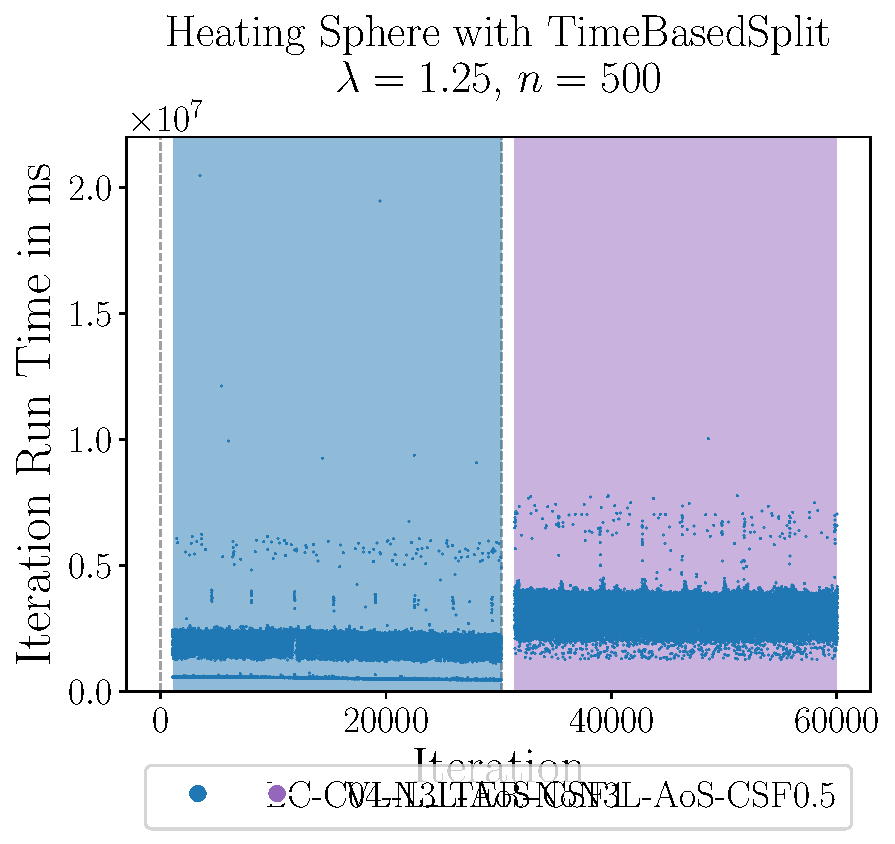
\includegraphics[width=\textwidth]{./Figures/plots/heating-sphere_configs_good.pdf}
		\subcaption{Reduced number of tuning phases.}
	\end{subfigure}
	\begin{subfigure}[c]{0.5\textwidth}
		\centering
		% heating-sphere_dynamic_TimeBasedRegression_1.25_1500
		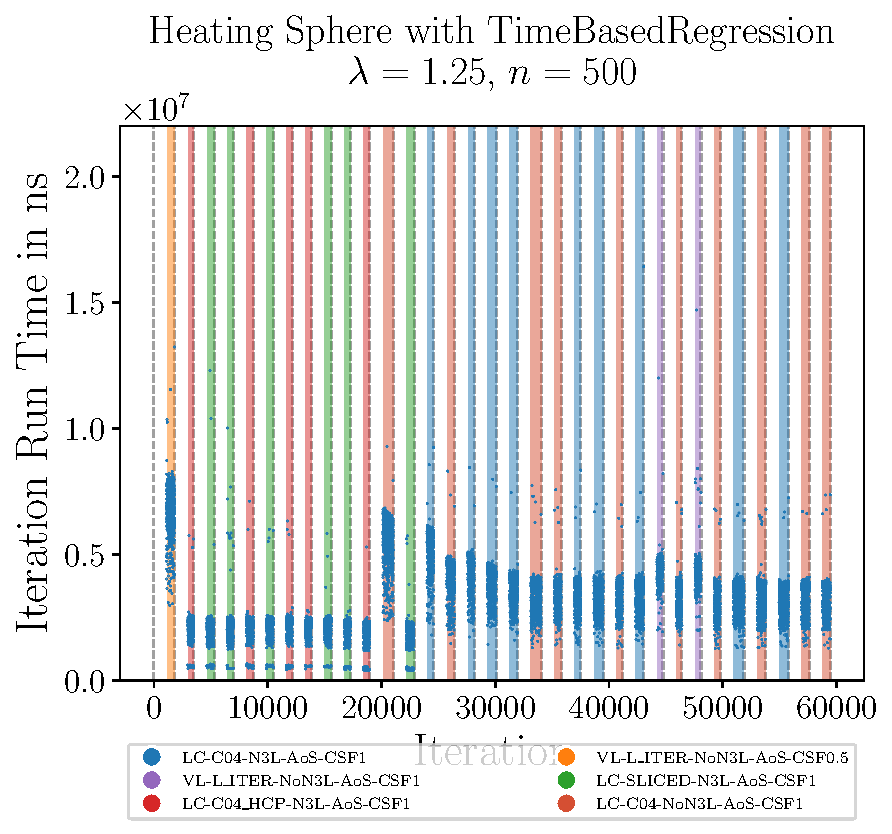
\includegraphics[width=\textwidth]{./Figures/plots/heating-sphere_configs_bad.pdf}
		\subcaption{Too many unneccessary tuning phases.}
	\end{subfigure}
	%	% TODO: maybe static run as comparison?
	\caption{Examples of trigger behavior in the heating-sphere scenario. [TODO]}
	\label{fig:hs_trigger_behavior}
\end{figure}

% TODO: Appendix plots:
% heating-sphere_dynamic_TimeBasedAverage_1.75_500
% heating-sphere_dynamic_TimeBasedSplit_1.25_250


\subsubsection{Speedup and Default Parameters}
The heating-sphere scenario experiences high variance in iteration runtimes, which directly influences the behavior of our trigger strategies, as shown in \autoref{fig:params_hs}. The triggers which should be unstable due to these variations are the \texttt{TimeBasedAverageTrigger}, \texttt{TimeBasedSimpleTrigger} and \texttt{TimeBasedRegressionTrigger}. However, results only show the poor performance of the latter two. The simple trigger under-performs the static approach by up to \qty{-41}{\percent} with a highly unfavourable \qty{99}{\percent} of all iterations being tuning iterations. Similarly, the regression approach leads to runtime increases across almost all tested combinations of $(\lambda, n)$.

The \texttt{TimeBasedAverageTrigger}, however, performs exceptionally well, with speedups of up to \qty{40}{\percent}, proportional to the decreased number of tuning iterations. % TODO: ...

In summary, it can be said that our approach is not suitable for the heating-sphere scenario. Considering that there is no clear indication of scenario change in runtime (cf. \autoref{sec:liveinfo_benchmarks}), this was expected.

%It should be noted, that the baseline run shows a larger share of tuning iterations than the previous scenario, since it used \num{60000} iterations (vs. \num{150000} in the equilibrium setting) while keeping the tuning interval at \num{5000} in both cases.

% TODO: split trigger
% TODO: explain why split higher speedup with same number of tuning its (better config choices)

% TODO: align plots vertically
\begin{figure}[htpb]
	\centering
	\begin{subfigure}{0.45\textwidth}
		\begin{tikzpicture}
			\begin{axis}[
					triggerplot,
					legend columns=2,
					ylabel={Speedup \%},
				]
				% Baseline
				\draw[linestyleE] (axis cs:0,0) -- (axis cs: 2,0);

				% TimeBasedSimple
				\addplot[linestyleD] coordinates{
						(1.25,-41)
						(1.5,-31)
						(1.75,-30)};
				% TimeBasedAverage 1000
				\addplot[linestyleA] coordinates{
						(1.25,29)
						(1.5,32)
						(1.75,23)};
				% TimeBasedAverage 500
				\addplot[linestyleB] coordinates{
						(1.25,37)
						(1.5,37)
						(1.75,26)};
				% TimeBasedAverage 250
				\addplot[linestyleC] coordinates{
						(1.25,31)
						(1.5,35)
						(1.75,40)};
				\legend{Simple,Avg-1000,Avg-500,Avg-250}
			\end{axis}
		\end{tikzpicture}
		%		\subcaption{Simple and Average Triggers}
	\end{subfigure}
	\hspace{0.05\textwidth}
	\begin{subfigure}{0.45\textwidth}
		\begin{tikzpicture}
			\begin{axis}[
					logtriggerplot,
					legend columns=2,
					ylabel={Tuning Iterations \%},
					ymode=log,
					ymin=1,
					ymax=100,
				]
				% Baseline
				\draw[linestyleE] (axis cs:0,25.13) -- (axis cs: 2,23.2);

				% TimeBasedSimple
				\addplot[linestyleD] coordinates{
						(1.25,99.78)
						(1.5,99.5)
						(1.75,98.58)};
				% TimeBasedAverage 1000
				\addplot[linestyleA] coordinates{
						(1.25,14.56)
						(1.5,11.6)
						(1.75,13.53)};
				% TimeBasedAverage 500
				\addplot[linestyleB] coordinates{
						(1.25,9.67)
						(1.5,7.73)
						(1.75,13.53)};
				% TimeBasedAverage 250
				\addplot[linestyleC] coordinates{
						(1.25,11.6)
						(1.5,9.67)
						(1.75,5.8)};
				\legend{Simple,Avg-1000,Avg-500,Avg-250}
			\end{axis}
		\end{tikzpicture}
		%		\subcaption{Simple and Average Triggers}
	\end{subfigure}
	\begin{subfigure}{0.45\textwidth}
		\begin{tikzpicture}
			\begin{axis}[
					triggerplot,
					ylabel={Speedup \%},
					ymin=-10,
				]
				% Baseline
				\draw[linestyleE] (axis cs:0,0) -- (axis cs: 2,0);

				% TimeBasedSplit 1000
				\addplot[linestyleA] coordinates{
						(1.25,30)
						(1.5,8)
						(1.75,8)};
				% TimeBasedSplit 500
				\addplot[linestyleB] coordinates{
						(1.25,8)
						(1.5,8)
						(1.75,8)};
				% TimeBasedSplit 250
				\addplot[linestyleC] coordinates{
						(1.25,8)
						(1.5,21)
						(1.75,6)};
				\legend{Split-1000,Split-500,Split-250}
			\end{axis}
		\end{tikzpicture}
		%		\subcaption{Split Trigger}
	\end{subfigure}
	\hspace{0.05\textwidth}
	\begin{subfigure}{0.45\textwidth}
		\begin{tikzpicture}
			\begin{axis}[
					logtriggerplot,
					ylabel={Tuning Iterations \%},
					ymode=log,
					ymin=1,
					ymax=100,
				]
				% Baseline
				\draw[linestyleE] (axis cs:0,25.13) -- (axis cs: 2,23.2);

				% TimeBasedSplit 1000
				\addplot[linestyleA] coordinates{
						(1.25,3.87)
						(1.5,1.93)
						(1.75,1.93)};
				% TimeBasedSplit 500
				\addplot[linestyleB] coordinates{
						(1.25,11.6)
						(1.5,1.93)
						(1.75,1.93)};
				% TimeBasedSplit 250
				\addplot[linestyleC] coordinates{
						(1.25,9.67)
						(1.5,3.87)
						(1.75,3.87)};
				\legend{Split-1000,Split-500,Split-250}
			\end{axis}
		\end{tikzpicture}
		%		\subcaption{Split Trigger}
	\end{subfigure}
	\begin{subfigure}{0.45\textwidth}
		\begin{tikzpicture}
			\begin{axis}[
					triggerplot,
					legend columns=2,
					ylabel={Speedup \%},
				]
				% Baseline
				\draw[linestyleE] (axis cs:0,0) -- (axis cs: 2,0);

				% TimeBasedRegression 2000
				%				\addplot[linestyleA] coordinates{
				%						(1.25,11)
				%						(1.5,-3)
				%						(1.75,0)}; % TODO

				% TimeBasedRegression 1500
				\addplot[linestyleB] coordinates{
						(1.25,-21)
						(1.5,-21)
						(1.75,-20)};

				% TimeBasedRegression 1000
				\addplot[linestyleC] coordinates{
						(1.25,-26)
						(1.5,-26)
						(1.75,-25)};

				% TimeBasedRegression 500		
				\addplot[linestyleD] coordinates{
						(1.25,-33)
						(1.5,9)
						(1.75,-31)};

				\legend{Reg-1500,Reg-1000,Reg-500}
			\end{axis}
		\end{tikzpicture}
		%		\subcaption{Regression Trigger}
	\end{subfigure}%
	\hspace{0.05\textwidth}
	\begin{subfigure}{0.45\textwidth}
		\begin{tikzpicture}
			\begin{axis}[
					logtriggerplot,
					legend columns=2,
					ylabel={Tuning Iterations \%},
					ymode=log,
					ymin=1,
					ymax=100,
				]
				% Baseline
				\draw[linestyleE] (axis cs:0,25.13) -- (axis cs: 2,23.2);

				% TimeBasedRegression 2000
				%				\addplot[linestyleA] coordinates{
				%						(1.25,36.73)
				%						(1.5,36.73)
				%						(1.75,0)}; %TODO

				% TimeBasedRegression 1500
				\addplot[linestyleB] coordinates{
						(1.25,40.6)
						(1.5,40.73)
						(1.75,39.78)};

				% TimeBasedRegression 1000
				\addplot[linestyleC] coordinates{
						(1.25,50.27)
						(1.5,50.27)
						(1.75,48.19)};

				% TimeBasedRegression 500		
				\addplot[linestyleD] coordinates{
						(1.25,64.07)
						(1.5,1.93) %TODO ?
						(1.75,59.93)};

				\legend{Reg-1500,Reg-1000,Reg-500}
			\end{axis}
		\end{tikzpicture}
		%		\subcaption{Regression Trigger}
	\end{subfigure}%
	\caption{Trigger behavior in the heating-sphere scenario, the numbers in the legends refer to the number of samples $n$ considered. The line in the background represents the baseline run. Note the logarithmic scale in the plots on the right hand side.}
	\label{fig:params_hs}
\end{figure}

The collected data suggests default parameters as presented in \autoref{tab:hs_defaults}.
\begin{table}[htpb]
	\centering
	\begin{tabular}{lcc}
		\toprule
		\textbf{Trigger}             & \textbf{Trigger factor $\lambda$} & \textbf{Number of samples $n$} \\ [0em]
		\midrule
		\texttt{TimeBasedSimple}     & not recommended                   & --                             \\
		\texttt{TimeBasedAverage}    & $1.5$                             & 500                            \\
		\texttt{TimeBasedSplit}      & $1.5$                             & 250                            \\
		\texttt{TimeBasedRegression} & not recommended                   & --                             \\
		\bottomrule
	\end{tabular}
	\caption{Suggested default parameters for the heating-sphere scenario.}
	\label{tab:hs_defaults}
\end{table}



\subsubsection{Optimality}
\autoref{fig:hs_optimality} shows the configuration selected by the best performing run for each trigger. The values again are given for all non-tuning iterations, compared to the configurations selected in the baseline run. Note that, e.g., the simple trigger displays better configuration fit than the averaging trigger; this is primarily due to tuning iterations being ignored. Additionally, not triggering a new tuning phase has a higher runtime impact than computing iterations with suboptimal configuration fit.

It can be seen that, particularly for the strategies triggering fewer tuning phases, i.e., the \texttt{TimeBasedAverageTrigger} and \texttt{TimeBasedSplitTrigger}, the configuration fit is suboptimal. For both, on average \qty{25}{\percent} of all non-tuning iterations were computed using a configuration that was not in the top 3 choices of the baseline run.


\begin{figure}[htpb]
	\begin{subfigure}{0.5\textwidth}
		\centering
		\begin{tikzpicture}
			\tikzset{
				barstyle1/.style={pattern color=tumblueaccmedium, draw=chaptertumblue,  pattern=crosshatch dots},
				barstyle2/.style={pattern color=tumblueaccmedium, draw=chaptertumblue, pattern=north east lines},
				barstyle3/.style={fill=tumblueaccmedium, draw=chaptertumblue},
				barstyle4/.style={pattern color=tumblueaccmedium, draw=chaptertumblue, pattern=vertical lines},
			}
			\def\barwidth{15pt}
			\begin{axis}[
					ybar stacked,
					height=0.8\textwidth,
					enlargelimits=0.15,
					ylabel={Selected Configuration in \unit{\percent}},
					xlabel={Trigger Strategy},
					%				ytick = \empty,
					symbolic x coords={Simple,Avg,Split,Reg},
					xtick=data,
					bar width=\barwidth,
					%				legend cell align=left,
					%				legend columns=1,
					%				legend style={at={(1.03,0.5)}, anchor=west, fill=none, draw=none, align=left},
					legend style={font=\small},
					legend cell align=center,
					legend columns=2,
					legend style={at={(0.5,1.03)}, anchor=south, fill=none, draw=none, align=center},
				]
				% TODO: align legend labels
				% TODO: regression?
				Top 1
				\addplot+[ybar, barstyle3] plot coordinates {(Simple,46) (Avg,27)
						(Split,10) (Reg,35)};

				% Top 2
				\addplot+[ybar, barstyle2] plot coordinates {(Simple,24) (Avg,9)
						(Split,15) (Reg,38)};

				% Top 3
				\addplot+[ybar, barstyle4] plot coordinates {(Simple,22) (Avg,36)
						(Split,33) (Reg,18)};

				% Other
				\addplot+[ybar, barstyle1] plot coordinates {(Simple,8) (Avg,28)
						(Split,42) (Reg,9)};

				\legend{Best,Second-Best,Third-Best,Other}
			\end{axis}
		\end{tikzpicture}
	\end{subfigure}%
	\begin{subfigure}{0.5\textwidth}
		\centering
		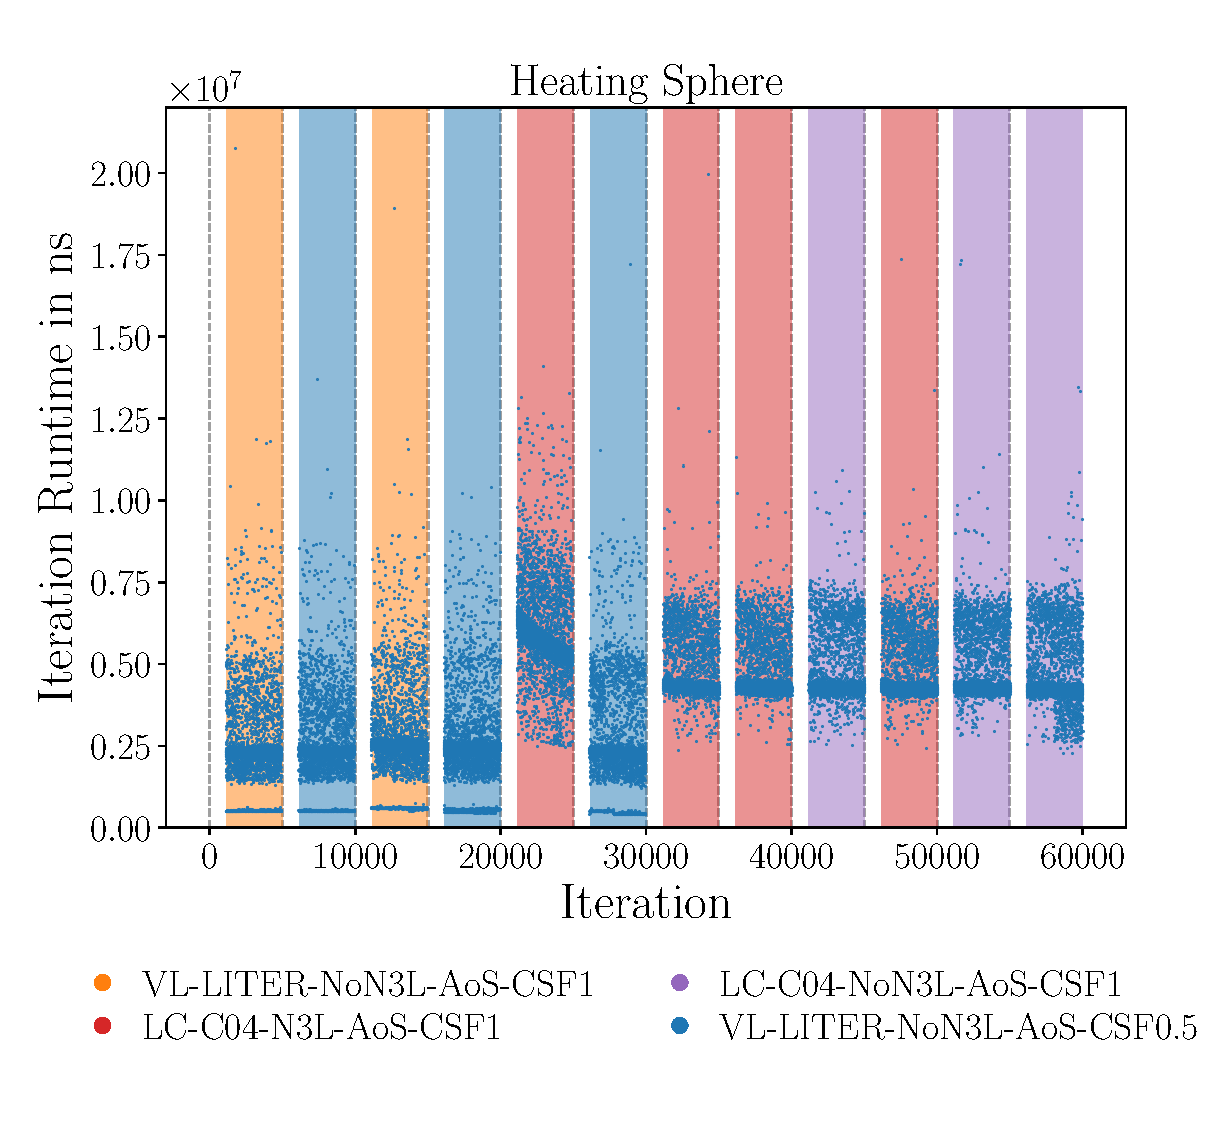
\includegraphics[width=\textwidth]{./Figures/plots/heating-sphere_configs_static.pdf}
		\vspace*{-1.075cm}
	\end{subfigure}
	\caption{Ranking of configurations selected by the best run in the heating-sphere scenario for each trigger strategy (left) and selected configurations in the baseline run (right).}
	\label{fig:hs_optimality}
\end{figure}
% TODO: update values

\newpage
%\subsection{Overview}
%%In the previous sections, the various trigger strategies were analyzed within each scenario. To better visualize the results of our benchmarks, \autoref{fig:overview_results_per_scenario} lays out the best speedup achieved, grouped by scenario.
%%The equilibrium scenario provides overall good conditions for application of our methods, as can seen by the speedup in all trigger strategies.
%%In the heating-sphere scenario, all strategies perform worse, except for the \texttt{TimeBasedSplitTrigger} which seems to be perfectly suited, with speedups of up to \qty{76}{\percent}.
%
%
%\begin{figure}[htpb]
%	\centering
%	%	\begin{tikzpicture}
%	%		\tikzset{
%	%			barstyle1/.style={pattern color=tumblueaccmedium, draw=chaptertumblue,  pattern=crosshatch dots},
%	%			barstyle2/.style={pattern color=tumblueaccmedium, draw=chaptertumblue, pattern=north east lines},
%	%			barstyle3/.style={fill=tumblueaccmedium, draw=chaptertumblue},
%	%			barstyle4/.style={pattern color=tumblueaccmedium, draw=chaptertumblue, pattern=vertical lines},
%	%		}
%	%		\def\barwidth{15pt}
%	%		\begin{axis}[
%	%				height=0.4\textwidth,
%	%				width=0.8\textwidth,
%	%				xlabel={Scenario},
%	%				ylabel={Best Speedup in \%},
%	%				enlarge x limits=0.25,
%	%				symbolic x coords={Equilibrium,Exploding Liquid,Heating Sphere},
%	%				xtick=data,
%	%				bar width=\barwidth,
%	%				ybar,
%	%				legend cell align=center,
%	%				legend columns=4,
%	%				legend style={at={(0.5,1.03)}, anchor=south, fill=none, draw=none, align=center},
%	%			]
%	%
%	%			\addlegendimage{legend image code/.code={
%	%						\draw[barstyle1,anchor=center, yshift=0.25ex] (0cm, -0.15cm)  rectangle (0.3cm,0.15cm);
%	%					}}
%	%			\addlegendentry{Simple}
%	%			\addlegendimage{legend image code/.code={
%	%						\draw[barstyle2, anchor=center, yshift=0.25ex] (0cm, -0.15cm)  rectangle (0.3cm,0.15cm);
%	%					}}
%	%			\addlegendentry{Average}
%	%			\addlegendimage{legend image code/.code={
%	%						\draw[barstyle3, anchor=center, yshift=0.25ex] (0cm, -0.15cm)  rectangle (0.3cm,0.15cm);
%	%					}}
%	%			\addlegendentry{Split}
%	%			\addlegendimage{legend image code/.code={
%	%						\draw[barstyle4, anchor=center, yshift=0.25ex] (0cm, -0.15cm)  rectangle (0.3cm,0.15cm);
%	%					}}
%	%			\addlegendentry{Regression}
%	%
%	%			% simple
%	%			\addplot[barstyle1] coordinates {
%	%					(Equilibrium,12)
%	%					(Exploding Liquid,0)
%	%					(Heating Sphere,-11)
%	%				};
%	%
%	%			% average
%	%			\addplot[barstyle2] coordinates {
%	%					(Equilibrium,47)
%	%					(Exploding Liquid,0)
%	%					(Heating Sphere,30)
%	%				};
%	%
%	%			% split
%	%			\addplot[barstyle3] coordinates {
%	%					(Equilibrium,46)
%	%					(Exploding Liquid,0)
%	%					(Heating Sphere,76)
%	%				};
%	%
%	%			% regression
%	%			\addplot[barstyle4] coordinates {
%	%					(Equilibrium,16)
%	%					(Exploding Liquid,0)
%	%					(Heating Sphere,11)
%	%				};
%	%
%	%			\coordinate (y) at (axis cs:Equilibrium,0);
%	%			\coordinate (x1) at (rel axis cs:0,0);
%	%			\coordinate (x2) at (rel axis cs:1,0);
%	%
%	%			%			\draw[gray, thin] (y -| x1) -- (y -| x2);
%	%		\end{axis}
%	%	\end{tikzpicture}
%	\caption{Average Speedup between unoptimized and optimized runs for the \texttt{TimeBasedAverage}, \texttt{TimeBasedSplit} and \texttt{TimeBasedRegression} strategies.}
%	\label{fig:overview_results_per_scenario}
%\end{figure}


%\section{Interaction with Tuning Strategies}
% TODO: How do results differ based on tuning strategy? Full-search vs. others

\section{Hybrid Triggers}
\label{sec:liveinfo_benchmarks}

Time-based approaches may not be suitable for all scenarios, if iteration runtime alone is not good enough indicator for scenario change. This was seen e.g. in the heating-sphere scenario. Since AutoPas provides additional live simulation statistics through its \texttt{LiveInfo} interface, these could be used in combination with iteration runtimes to find better strategies in detecting scenario change.
As a motivation of this approach, \autoref{fig:liveinfo_heating_sphere} shows an exemplary run in the heating-sphere scenario.
Using static containers, the initial optimal configuration is \texttt{VL-List\_Iter-NoN3L-AoS}, later on it changes to \texttt{LC-C04-N3L-AoS-CSF1}. \cite{Newcome2025}
The iteration runtime does not change, even tough a better configuration is available. Considering that the particles are packed closely in the inital phase and expand outwards, the decrease in particle density, as reported by the \texttt{maxDensity} statistics is consistent with expectations. It would therefore be a reasonable trigger input, as it shows clear indication of the shift towards a different simulation state.

%TODO: timebasedsplit 1.25, 250 is opposite is good example, n=500 even better

% TODO: fix figure height
% TODO: results not consistent with assumption
\begin{figure}[htpb]
	\centering
	\begin{subfigure}{0.5\textwidth}
		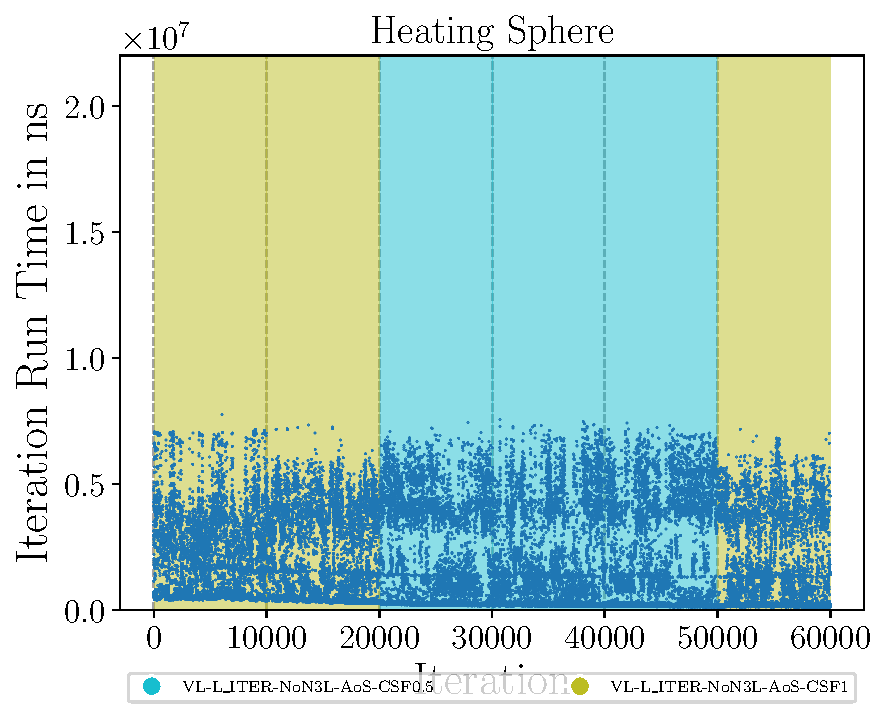
\includegraphics[width=\textwidth]{./plots/hs_vl_list_iter-non3l-aos_configs.pdf}
	\end{subfigure}%
	\begin{subfigure}{0.5\textwidth}
		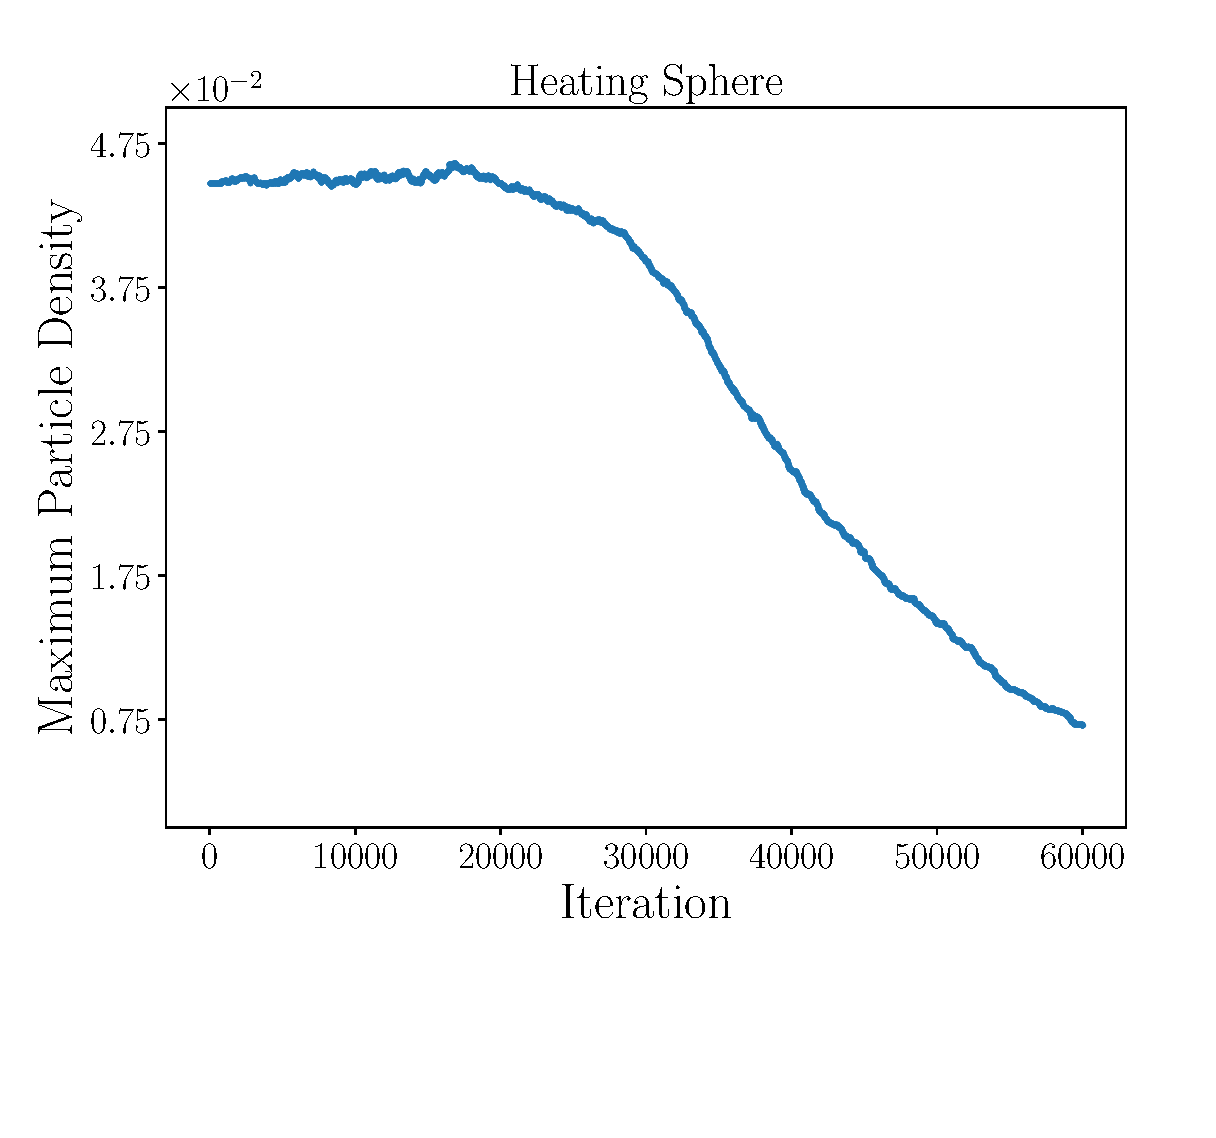
\includegraphics[width=\textwidth]{./plots/hs_vl_list_iter-non3l-aos_max_density.pdf}
	\end{subfigure}
	\begin{subfigure}{0.5\textwidth}
		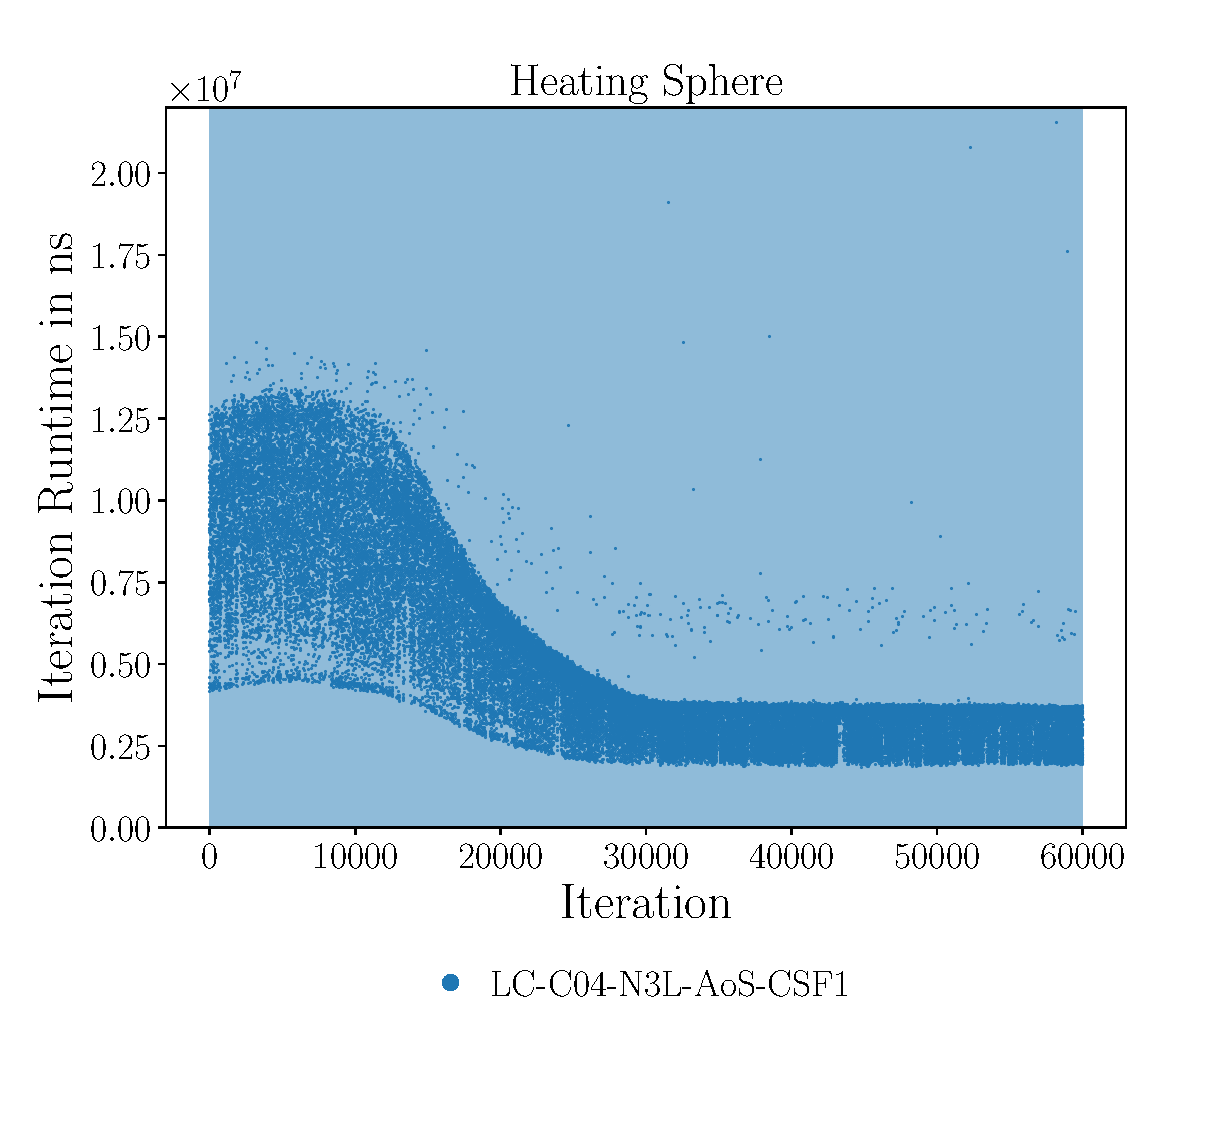
\includegraphics[width=\textwidth]{./plots/hs_lc_c04_n3l-aos-csf1_configs.pdf}
	\end{subfigure}%
	\begin{subfigure}{0.5\textwidth}
		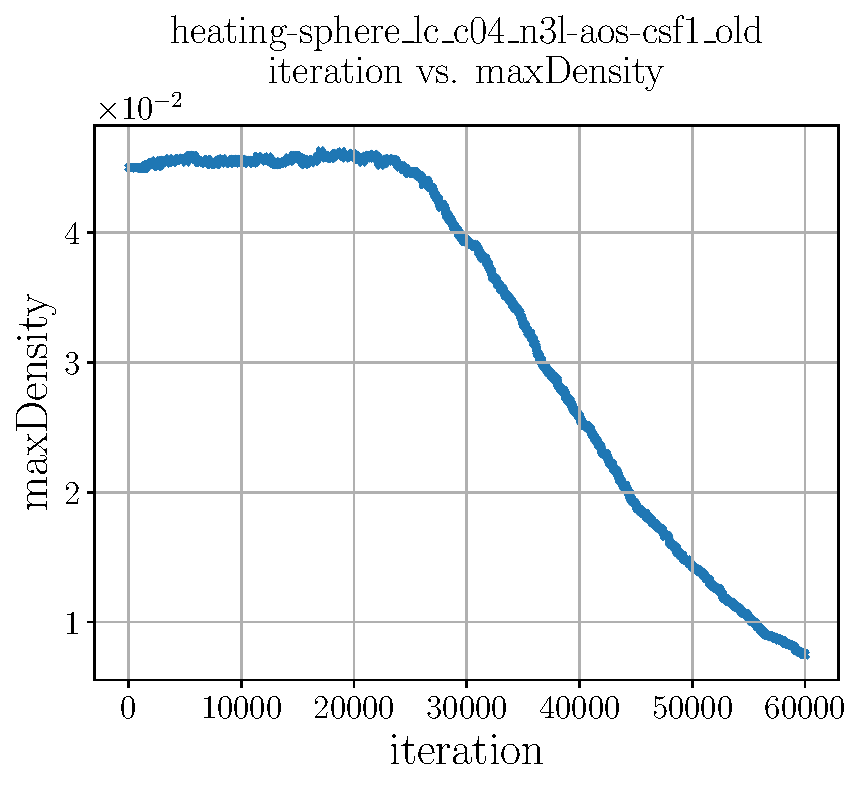
\includegraphics[width=\textwidth]{./plots/hs_lc_c04_n3l-aos-csf1_max_density.pdf}
	\end{subfigure}
	\caption{Iteration runtime (left) and the maximum particle density (right). The top row shows a run with the single configuration \texttt{VL-List\_Iter-NoN3L-AoS}, the bottom row shows \texttt{LC-C04-N3L-AoS-CSF1}}
	\label{fig:liveinfo_heating_sphere}
\end{figure}





